% !TEX root = ../main.tex
%-------------------------------------------------------------------------------
\section{Case Study: Access Control Device}
%-------------------------------------------------------------------------------
In this section, we evaluate the effectiveness of \texttt{DepthFake} attacks on a commercial access control device in the real world as a case study.

\begin{figure}[pt]
	\centerline{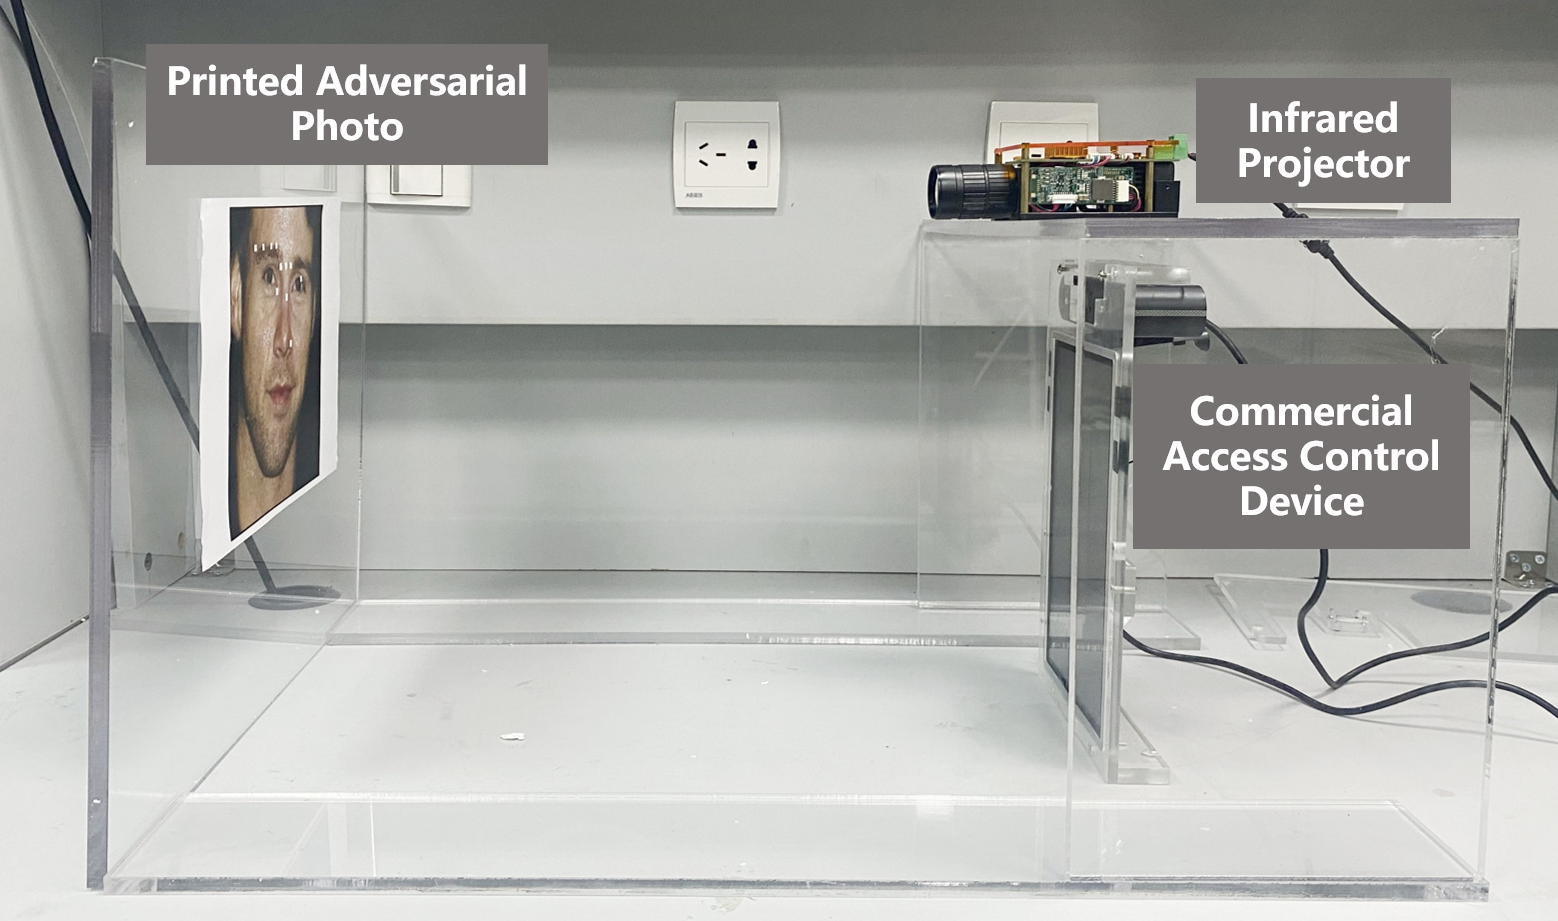
\includegraphics[width = 0.48\textwidth]{figures/commercial_setup.png}}
	\vspace{-0.1in}
	\caption{Experimental setup against an commercial access control device. An infrared projector is used to project a structured light scatter pattern onto an adversarial photo of a legitimate user present in front of the target module.}
	\vspace{-0.1in}
	\label{setup_2}
\end{figure}
\begin{figure}[pt]
	\centerline{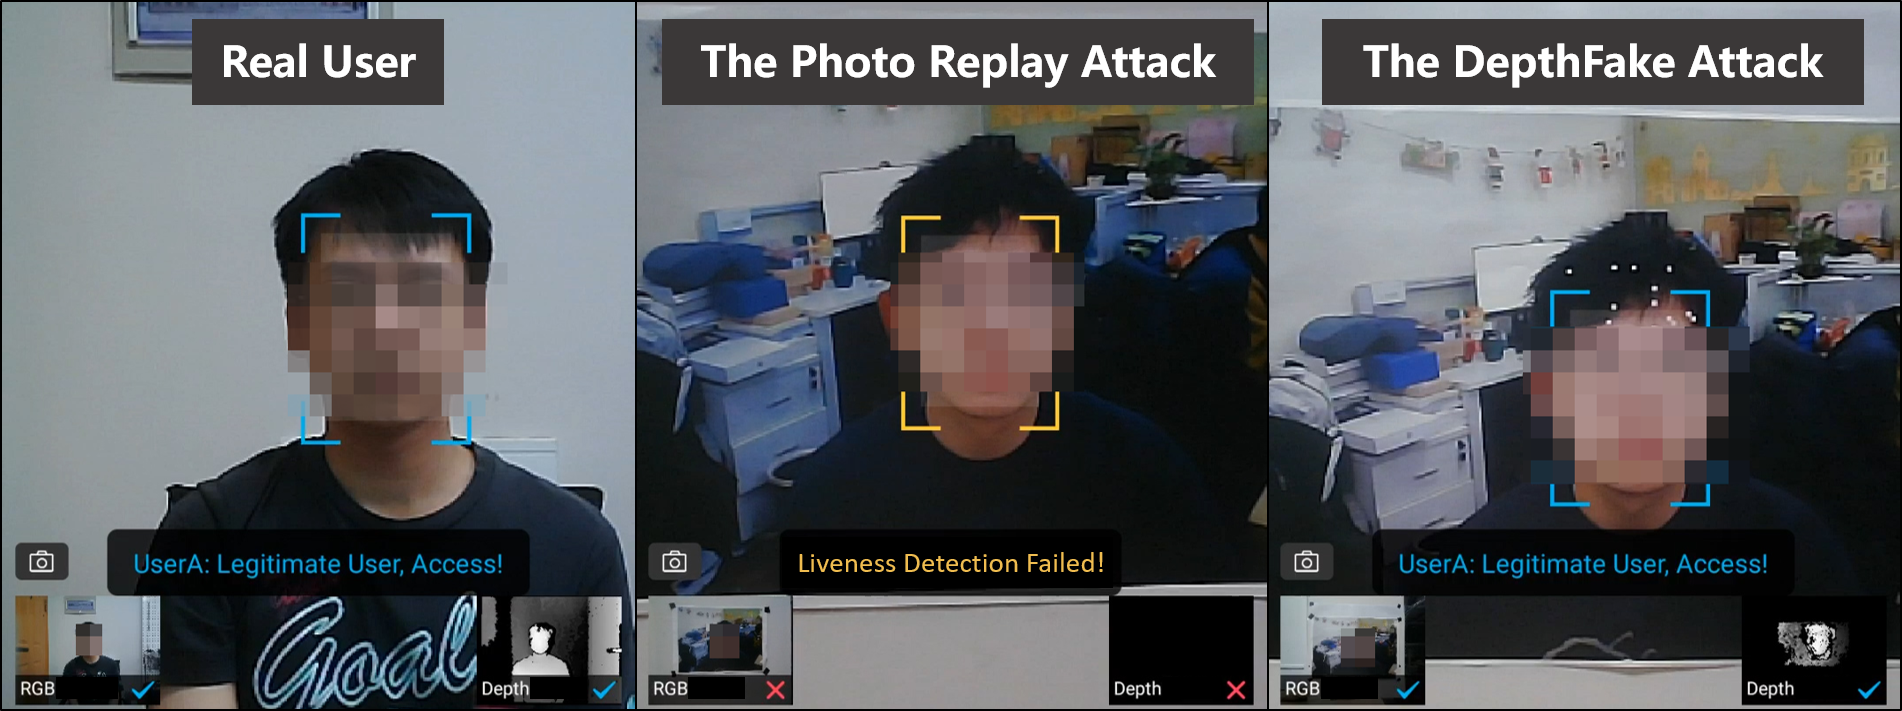
\includegraphics[width = 0.48\textwidth]{figures/commercial_compare.png}}
	\vspace{-0.1in}
	\caption{An illustration of the face authentication results on the real user, the photo replay attack and the \texttt{DepthFake} attack.}
	\vspace{-0.1in}
	\label{compare}
\end{figure}

\begin{table}[pt]
	\caption{Attack Effectiveness of \texttt{DepthFake} on a Commercial Access Control Device}
	\vspace{-0.15in}
	\begin{center}
		\setlength{\tabcolsep}{2mm}{
			\renewcommand{\arraystretch}{1.2} 
			\begin{tabular}{c|c|c}
				\hline
				\textbf{Victim Users} & \textbf{Attack Success Rate} & \makecell[c]{\textbf{Max Continues Frames}\\ \textbf{Under Attack}} \\
				\hline
				\hline
				Person A & $52.2\%$ & 9\\
				\hline
				Person B & $62.4\%$ & 12\\
				\hline
				Person C & $61.1\%$ & 15\\
				\hline
				Person D & $45.5\%$ & 6\\
				\hline
				Person E & $82.0\%$ & 26\\
				\hline
		\end{tabular}}
		\label{commercial_asr}
	\end{center}
	\vspace{-0.15in}
\end{table}

\subsection{Experimental Setup}
\textbf{Target Device.} We analyze a commercial access control device Baidu Rattlesnake Application Kit equipped with Baidu Face Authentication SDK and an Orbbec Astra depth camera, which has been used in airports, metros, banks, and other critical infrastructures in China~\cite{baidu_customer}.
The liveness detection module is set to RGB-D mode with default thresholds  (i.e., RGB:0.5, Depth:0.5).

\textbf{Attack Devices.} For Depth attacks, we use an infrared projector DLP4500SL02 Evaluation Module and place it on the top of the camera at a distance of $20~mm$. For RGB attacks, we use a $400~mm\times300~mm$ printed adversarial photo of the legitimate user and place it in front of the target device with a distance of $500~mm$, as shown in Fig.~\ref{setup_2}.

% \subsection{Attack Methodology}
%The \texttt{DepthFake} attack consists of two steps: (1) modulating the desired scatter pattern from the victim's photo and generating the RGB adversarial example, and (2) launching the RGB-D attack to spoof the target device.

%For the scatter pattern modulation, we first use an infrared camera to extract the template scatter pattern of the target device. Then, we obtain the victim's photo, estimate its depth information and modulate it to the desired scatter pattern. 
%For the RGB adversarial attack, we use the victim's photo to generate the adversarial example, then print and put it in front of the target device. 

\subsection{Attack Performance}
We conduct experiments with the Baidu Rattlesnake Application Kit on five legitimate users.
Before experiments, we first generate the users' modulated structured light scatter patterns and their RGB adversarial photos.
During attacks, we cover the scatter projector of the target depth camera and use the infrared projector to project the modulated scatter pattern on the printed adversarial photo. Then, the depth camera will feed the captured RGB and depth images into the face authentication system of the target device, and output the authentication results.

An illustration of the real-world \texttt{DepthFake} attack against the commercial access control device is shown in Fig.~\ref{compare}. The results show that 3D liveness detection can defend against the naive photo replay attack, but is not effective when against the \texttt{DepthFake} attack. 

To illustrate the effectiveness of \texttt{DepthFake} attacks quantitatively, we launch attacks for 1000 frames per user and record the attack success rate and the max continuous attack success frames.
As shown in Tab.~\ref{commercial_asr}, we find that our attack is effective against five users, and can achieve an average attack success rate of $60.64\%$. 
Meanwhile, the results demonstrate that our attack can succeed over 6 continuous frames, indicating the feasibility of our attacks against commercial products utilizing multiple frames for liveness detection.  The demo of the \texttt{DepthFake} against the target access control device can be found at https://sites.google.com/view/depthfake.

